Argomento del corso: preparare gli studenti alla scrittura di algoritmi \textit{efficienti}.
Un algoritmo è definito \textit{inefficiente} se la sua complessità è esponenziale.\\
La maggior parte dei problemi non artefatti sono risolvibili in tempi esponenziali o polinomiali.

\section{Grafi}
I grafi sono \textit{modelli} utilizzati per semplificare lo studio di problemi e la ricerca di soluzioni ad essi.
\subsection{Grafi e Alberi}
I grafi sono considerabili come una "sovraclasse" degli \textit{alberi}. \\
Le differenze principali sono:
\begin{itemize}
	\item i grafi non sono necessariamente connessi (non tutti i nodi sono collegati);
	\item i grafi possono avere cicli.
\end{itemize}
Appare chiaro che utilizzare grafi diversi dagli alberi è molto utile se si necessita di rappresentare strutture non gerarchiche. \\
Notare inoltre che, al contrario dei grafi, in un albero il numero complessivo di archi è necessariamente $n-1$, dove \textit{n} è definito come il numero totale di nodi.

\subsection{Composizione}
Sono composti da due entità:
\begin{itemize}
	\item \textbf{nodi}: anche detti \textit{vertici}; il loro insieme V è rappresentato come insieme dei loro nomi. Generalmente, la cardinalità di V è indicata con \textit{n}.
	\item \textbf{archi}: collegano i vari nodi. L'insieme E degli archi di un grafo è rappresentato dai nomi delle coppie di nodi che essi collegano. Possono essere unidirezionali o bidirezionali.
\end{itemize}
Si distinguono in \textit{grafi diretti} (con archi unidirezionali) e \textit{grafi indiretti} (con archi bidirezionali).
\paragraph{Pozzo.}
In un grafo diretto, si definisce \textit{pozzo} un nodo da cui non esce nessun arco.
\paragraph{Pozzo universale.}
In un grafo diretto, si definisce \textit{pozzo universale} un pozzo verso cui, direttamente o indirettamente, puntano tutti gli altri nodi.
\paragraph{Esercizio.}
Dato un grafo, trovare l'algoritmo che restituisce - in $O(n)$ - \textit{vero} se il nodo in input rappresenta un pozzo universale. \\
\textbf{Soluzione}:
\begin{algorithm}
	\caption{Algoritmo vero per X rappresentate un pozzo}\label{alg:pozzo-x}
	\begin{algorithmic}[1]
		\Function{pozzo}{$x$}
			\For {$i \gets 1$ to $n$}
				\If {($i \neq x$) and ($M[i,x] = 0$ or $M[x,i] = 1$)}
					\State \Return falso
				\EndIf
			\EndFor
			\State \Return vero
		\EndFunction
	\end{algorithmic}
\end{algorithm} \hfill \\
Dove \textit{M[x,y]} indica l'arco che lega il nodo \textit{x} al nodo \textit{y} nella rappresentazione a matrice. \\
La complessità è di $O(n)$ perché la verifica di $M[x,i]$ (o $M[i,x]$) costa $O(1)$. Differente è invece il caso in cui si analizza il caso in cui il grafo sia rappresentato tramite liste di adiacenze, che porterebbe ad una complessità di $O(n^2)$.

\subsection{Tipo}
Esistono due tipi di grafi:
\begin{itemize}
    \item \textbf{Grafi diretti}: i cui archi hanno una direzione. Possono rappresentare, quindi, sia grafi (mono)direzionali, che bidirezionali;
    \item \textbf{Grafi indiretti}: i cui archi non hanno direzione. Possono rappresentare unicamente grafi bidirezionali.
\end{itemize}

\newpage

\subsection{Rappresentazioni}
\subsubsection{Rappresentazione semplice (standard)}
\begin{center}
    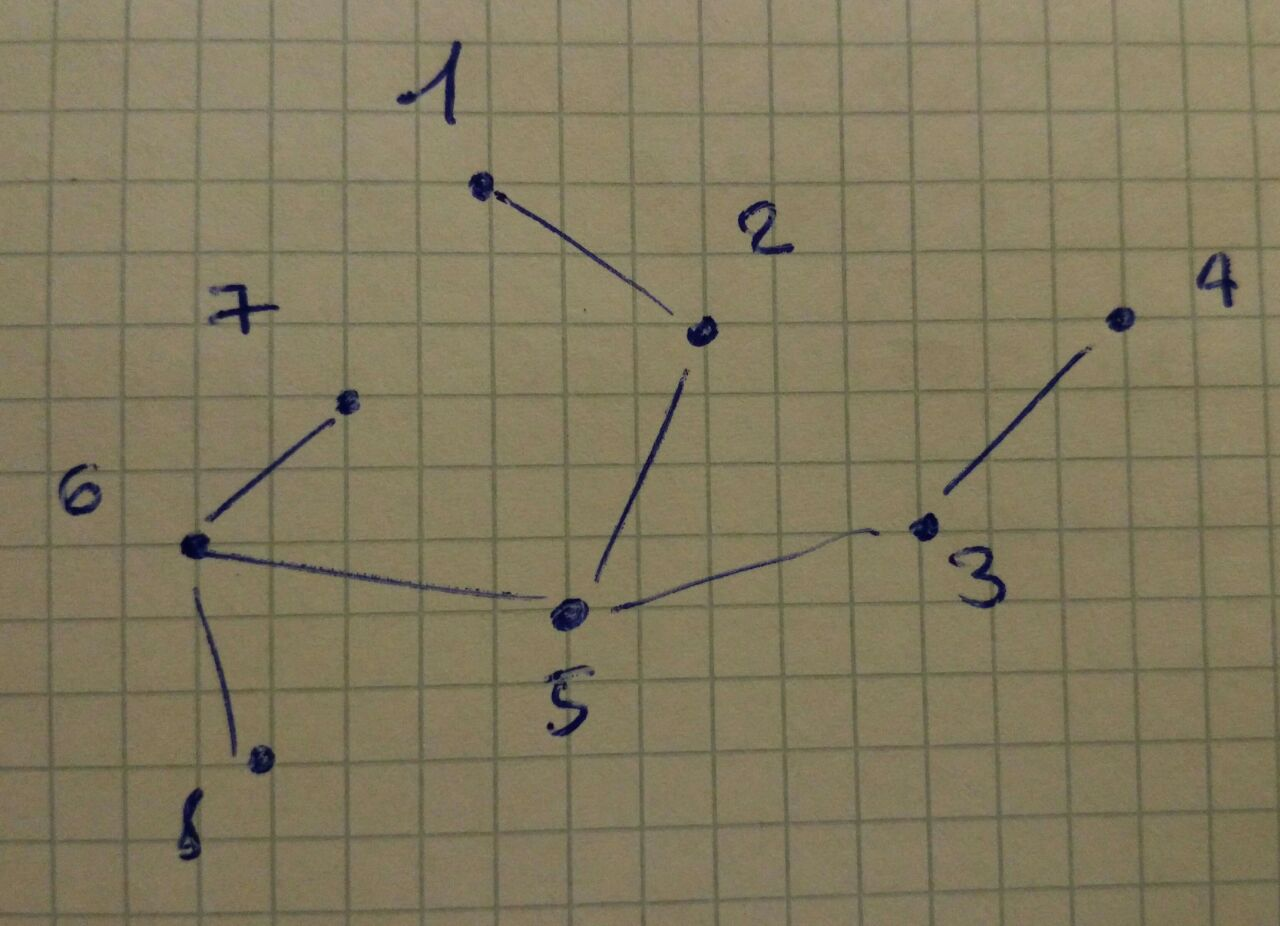
\includegraphics[width=.4\textwidth]{res/rappresentazione-standard.jpg} \hfill
\end{center}
\subsubsection{Rappresentazione tramite matrice}
\begin{center}
    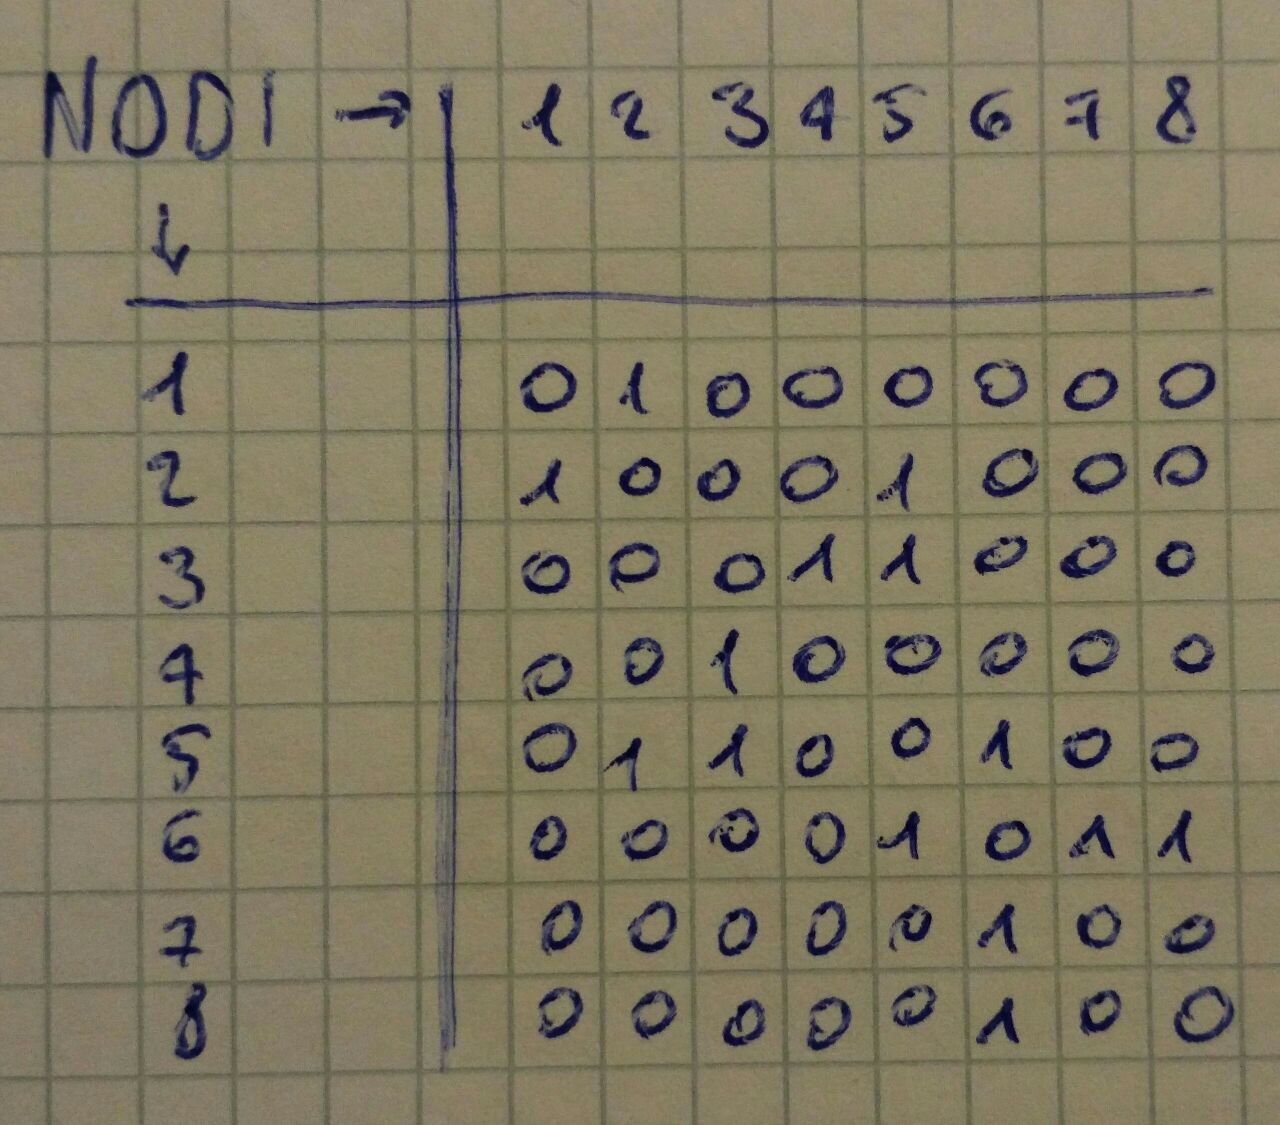
\includegraphics[width=.4\textwidth]{res/rappresentazione-matrice.jpg} \hfill
\end{center}
\subsubsection{Rappresentazione tramite lista di adiacenze}
\begin{center}
    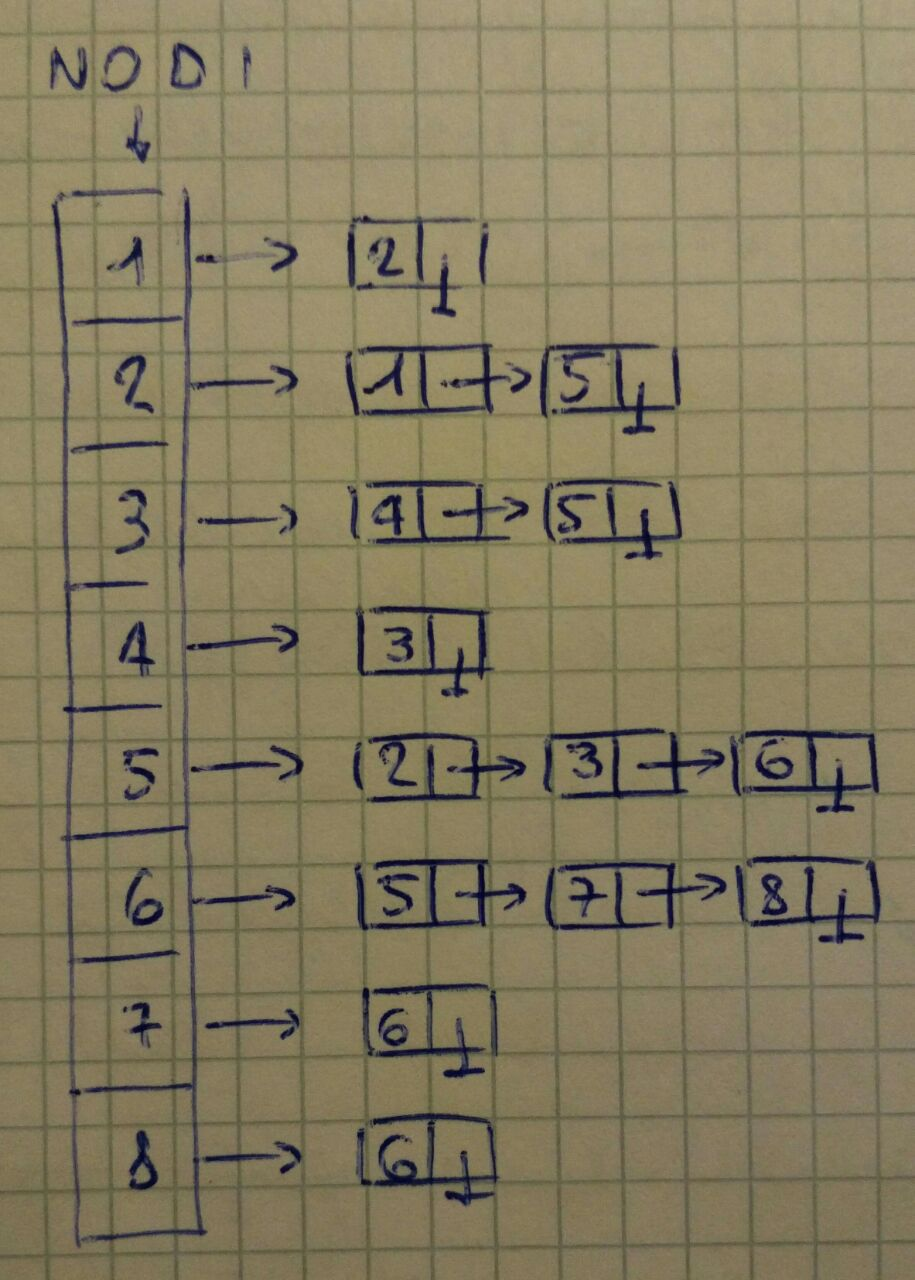
\includegraphics[width=.4\textwidth]{res/rappresentazione-lista-adiacenze.jpg} \hfill
\end{center}